\documentclass[landscape,a0paper,fontscale=0.292]{baposter}

\usepackage[vlined]{algorithm2e}
\usepackage{times}
\usepackage{calc}
\usepackage{url}
\usepackage{graphicx}
\usepackage{amsmath}
\usepackage{amssymb}
\usepackage{relsize}
\usepackage{multirow}
\usepackage{booktabs}

\usepackage{graphicx}
\usepackage{multicol}
\usepackage[T1]{fontenc}
\usepackage{ae}

\graphicspath{{images/}}

 %%%%%%%%%%%%%%%%%%%%%%%%%%%%%%%%%%%%%%%%%%%%%%%%%%%%%%%%%%%%%%%%%%%%%%%%%%%%%%%%
 %%%% Some math symbols used in the text
 %%%%%%%%%%%%%%%%%%%%%%%%%%%%%%%%%%%%%%%%%%%%%%%%%%%%%%%%%%%%%%%%%%%%%%%%%%%%%%%%
 % Format 
 \newcommand{\RotUP}[1]{\begin{sideways}#1\end{sideways}}


 %%%%%%%%%%%%%%%%%%%%%%%%%%%%%%%%%%%%%%%%%%%%%%%%%%%%%%%%%%%%%%%%%%%%%%%%%%%%%%%%
 % Multicol Settings
 %%%%%%%%%%%%%%%%%%%%%%%%%%%%%%%%%%%%%%%%%%%%%%%%%%%%%%%%%%%%%%%%%%%%%%%%%%%%%%%%
 \setlength{\columnsep}{0.7em}
 \setlength{\columnseprule}{0mm}


 %%%%%%%%%%%%%%%%%%%%%%%%%%%%%%%%%%%%%%%%%%%%%%%%%%%%%%%%%%%%%%%%%%%%%%%%%%%%%%%%
 % Save space in lists. Use this after the opening of the list
 %%%%%%%%%%%%%%%%%%%%%%%%%%%%%%%%%%%%%%%%%%%%%%%%%%%%%%%%%%%%%%%%%%%%%%%%%%%%%%%%
 \newcommand{\compresslist}{%
 \setlength{\itemsep}{1pt}%
 \setlength{\parskip}{0pt}%
 \setlength{\parsep}{0pt}%
 }


 %%%%%%%%%%%%%%%%%%%%%%%%%%%%%%%%%%%%%%%%%%%%%%%%%%%%%%%%%%%%%%%%%%%%%%%%%%%%%%
 % Formating
 \newcommand{\Matrix}[1]{\begin{bmatrix} #1 \end{bmatrix}}
 \newcommand{\Vector}[1]{\begin{pmatrix} #1 \end{pmatrix}}

 \newcommand*{\norm}[1]{\mathopen\| #1 \mathclose\|}% use instead of $\|x\|$
 \newcommand*{\abs}[1]{\mathopen| #1 \mathclose|}% use instead of $\|x\|$
 \newcommand*{\normLR}[1]{\left\| #1 \right\|}% use instead of $\|x\|$

 \newcommand*{\SET}[1]  {\ensuremath{\mathcal{#1}}}
 \newcommand*{\FUN}[1]  {\ensuremath{\mathcal{#1}}}
 \newcommand*{\MAT}[1]  {\ensuremath{\boldsymbol{#1}}}
 \newcommand*{\VEC}[1]  {\ensuremath{\boldsymbol{#1}}}
 \newcommand*{\CONST}[1]{\ensuremath{\mathit{#1}}}

 \DeclareMathOperator*{\argmax}{arg\,max}
 \DeclareMathOperator*{\diag}{diag}
 \DeclareMathOperator*{\argmin}{arg\,min}
 \DeclareMathOperator*{\vectorize}{vec}
 \DeclareMathOperator*{\reshape}{reshape}

 %-----------------------------------------------------------------------------
 % Differentiation
 \newcommand*{\Nabla}[1]{\nabla_{\!#1}}

 \renewcommand*{\d}{\mathrm{d}}
 \newcommand*{\dd}{\partial}

 \newcommand*{\At}[2]{\ensuremath{\left.#1\right|_{#2}}}
 \newcommand*{\AtZero}[1]{\At{#1}{\pp=\VEC 0}}

 \newcommand*{\diffp}[2]{\ensuremath{\frac{\dd #1}{\dd #2}}}
 \newcommand*{\diffpp}[3]{\ensuremath{\frac{\dd^2 #1}{\dd #2 \dd #3}}}
 \newcommand*{\diffppp}[4]{\ensuremath{\frac{\dd^3 #1}{\dd #2 \dd #3 \dd #4}}}
 \newcommand*{\difff}[2]{\ensuremath{\frac{\d #1}{\d #2}}}
 \newcommand*{\diffff}[3]{\ensuremath{\frac{\d^2 #1}{\d #2 \d #3}}}
 \newcommand*{\difffp}[3]{\ensuremath{\frac{\dd\d #1}{\d #2 \dd #3}}}
 \newcommand*{\difffpp}[4]{\ensuremath{\frac{\dd^2\d #1}{\d #2 \dd #3 \dd #4}}}

 \newcommand*{\diffpAtZero}[2]{\ensuremath{\AtZero{\diffp{#1}{#2}}}}
 \newcommand*{\diffppAtZero}[3]{\ensuremath{\AtZero{\diffpp{#1}{#2}{#3}}}}
 \newcommand*{\difffAt}[3]{\ensuremath{\At{\difff{#1}{#2}}{#3}}}
 \newcommand*{\difffAtZero}[2]{\ensuremath{\AtZero{\difff{#1}{#2}}}}
 \newcommand*{\difffpAtZero}[3]{\ensuremath{\AtZero{\difffp{#1}{#2}{#3}}}}
 \newcommand*{\difffppAtZero}[4]{\ensuremath{\AtZero{\difffpp{#1}{#2}{#3}{#4}}}}

 %-----------------------------------------------------------------------------
 % Defined
 % How should the defined operator look like (:= or ^= ==)
 % (I want back my :=, it is so much better than ^= because (1) it has a
 % direction and (2) everyone here uses it.)
 %
 % Use :=
 %\newcommand*{\defined}{\ensuremath{\mathrel{\mathop{:}}=}}
 %\newcommand*{\definedRight}{\ensuremath{=\mathrel{\mathop{:}}}}
 % Use ^=
 \newcommand*{\defined}{\ensuremath{\triangleq}}
 \newcommand*{\definedRight}{\ensuremath{\triangleq}}
 % Use = with three bars
 %\newcommand*{\defined}{\ensuremath{?}}
 %\newcommand*{\definedRight}{\ensuremath{?}}

 %%%%%%%%%%%%%%%%%%%%%%%%%%%%%%%%%%%%%%%%%%%%%%%%%%%%%%%%%%%%%%%%%%%%%%%%%%%%%%
 % Symbols used in the paper

 %-----------------------------------------------------------------------------
 % The Methods
 \newcommand*{\ICIA}{\emph{ICIA}}
 \newcommand*{\CoDe}{\emph{CoDe}}
 \newcommand*{\LinCoDe}{\emph{LinCoDe}}
 \newcommand*{\CoNe}{\emph{CoNe}}
 \newcommand*{\CoLiNe}{\emph{CoLiNe}}
 \newcommand*{\LinCoLiNe}{\emph{LinCoLiNe}}

 % inter eye distance
 \newcommand*{\ied}{IED}

 %-----------------------------------------------------------------------------
 % Koerper
 %%\newcommand*{\RR}{\mathbb{R}}
 %\newcommand*{\RR}{{I\hspace{-3.5pt}R}}
 %\newcommand*{\RR}{{\mathrm{I\hspace{-2.7pt}R}}}

 \font\dsfnt=dsrom12

 \DeclareSymbolFont{nark}{U}{dsrom}{m}{n}
 \DeclareMathSymbol{\NN}{\dsfnt}{nark}{`N}
 \DeclareMathSymbol{\RR}{\dsfnt}{nark}{`R}
 \DeclareMathSymbol{\ZZ}{\dsfnt}{nark}{`Z}

 %-----------------------------------------------------------------------------
 % Domains
 \newcommand*{\D}{\mathcal{D}}
 \newcommand*{\I}{\mathcal{I}}

 %-----------------------------------------------------------------------------
 % Texture coordinates
 \newcommand*{\rr}{\VEC{r}}

 %-----------------------------------------------------------------------------
 % Parameters
 \newcommand*{\pt}{\VEC{\tau}}
 \newcommand*{\pr}{\VEC{\rho}}
 \newcommand*{\pp}{\VEC{p}}
 \newcommand*{\qq}{\VEC{q}}
 \newcommand*{\xx}{\VEC{x}}
 \newcommand*{\deltaq}{\Delta \qq}
 \newcommand*{\deltap}{\Delta \pp}
 \newcommand*{\zz}{\VEC{z}}
 \newcommand*{\pa}{\VEC{\alpha}}
 \newcommand*{\qa}{\VEC{\alpha}}
 \newcommand*{\pb}{\VEC{\beta}}

 %-----------------------------------------------------------------------------
 % Optimal appearance parameters
 \newcommand*{\pbh}[1]{\ensuremath{\hat{\pb}({#1})}}

 %-----------------------------------------------------------------------------
 % Warp basis
 \newcommand*{\M}[1]{\ensuremath{M({#1})}}
 \newcommand*{\LL}[1]{\ensuremath{L({#1})}}

 %-----------------------------------------------------------------------------
 % Matrices of the texture model
 \newcommand*{\AM}[1]{\ensuremath{\Lambda(#1)}}               % Lambda(beta) 
 \newcommand*{\AMr}[2]{\ensuremath{\Lambda(#1; #2)}}        % Lambda(r, beta)

 \newcommand*{\As}{A}         % Continuous Basis symbol
 \newcommand*{\afs}{a}        % Continuous mean symbol
 \newcommand*{\A}[1]{\As(#1)}         % Continuous Basis
 \newcommand*{\af}[1]{\afs(#1)}        % Continuous mean


 %-----------------------------------------------------------------------------
 % Matrices of the shape model
 \newcommand*{\MU}{\VEC{\mu}}
 \newcommand*{\MM}{\MAT{M}}

 %-----------------------------------------------------------------------------
 %% The project out matrix and operator
 \newcommand*{\INT}{\MAT{P}}
 \newcommand*{\INTf}{P}

 %-----------------------------------------------------------------------------
 % The identity matrix
 \newcommand*{\EYEtwo}{\Matrix{1 & 0\\0&1}}
 \newcommand*{\EYE}{\MAT E}
 \newcommand*{\EYEf}{E}

 % Wether to use subscripts or brackets for some function arguments
 % can be decided by commenting out the corresponding functions underneath
 %-----------------------------------------------------------------------------
 % Mapping
 \newcommand*{\Cs}[1]{\ensuremath{C^{#1}}} % C symbol
 \newcommand*{\C}[2]{\ensuremath{C^{#1}(#2)}} % Use C with brackets

 %-----------------------------------------------------------------------------
 % Objective function
 \newcommand*{\Fs}{\ensuremath{F}}              % F symbol
 \newcommand*{\F}[1]{\ensuremath{\Fs(#1)}}       % Use F with brackets    F(q)

 %-----------------------------------------------------------------------------
 % Approximated objective functions
 \newcommand*{\FFs}{\tilde{F}}                     % ~F symbol
 \newcommand*{\FF}[1]{\ensuremath{\FFs(#1)}}       % Use ~F with brackets    F(q)

 %-----------------------------------------------------------------------------
 % residual function
 \newcommand*{\es}{\ensuremath{f}}              % R symbol

 \newcommand*{\e}[1]{\ensuremath{\es(#1)}}         % R(q)
 \newcommand*{\er}[2]{\ensuremath{\es(#1; #2)}}    % R(r; q)

 %-----------------------------------------------------------------------------
 % Approximated residual functions
 \newcommand*{\ees}{\tilde{f}}                       % ~R symbol
 \newcommand*{\ee}[1]{\ensuremath{\ees(#1)}}       % ~R(q)
 \newcommand*{\eer}[2]{\ensuremath{\ees(#2; #1)}}  % ~R(r; q)

 %-----------------------------------------------------------------------------
 % Warps
 \newcommand*{\Vs}{\ensuremath{V}}
 \newcommand*{\VLins}{\ensuremath{\Vs^{\text{Ortho}}}}
 \newcommand{\VModels}{\ensuremath{\Vs^{\text{Model}}}}
 \newcommand*{\Ws}{\ensuremath{W}}

 \newcommand{\V}[1]{\ensuremath{\Vs(#1)}}
 \newcommand{\VModel}[1]{\ensuremath{\VModels(#1)}}
 \newcommand{\Vr}[2]{\ensuremath{\Vs(#1; #2)}}
 \newcommand{\VInvr}[2]{\ensuremath{\Vs^{-1}(#1; #2)}}
 \newcommand{\VrLin}[2]{\ensuremath{\VLins(#1; #2)}}
 \newcommand{\W}[1]{\ensuremath{\Ws(#1)}}
 \newcommand{\Winv}[1]{\ensuremath{\Ws^{-1}(#1)}}
 \newcommand{\Wr}[2]{\ensuremath{\Ws(#1; #2)}}


%%%%%%%%%%%%%%%%%%%%%%%%%%%%%%%%%%%%%%%%%%%%%%%%%%%%%%%%%%%%%%%%%%%%%%%%%%%%%
%% Begin of Document
%%%%%%%%%%%%%%%%%%%%%%%%%%%%%%%%%%%%%%%%%%%%%%%%%%%%%%%%%%%%%%%%%%%%%%%%%%%%%
\begin{document}
%%%%%%%%%%%%%%%%%%%%%%%%%%%%%%%%%%%%%%%%%%%%%%%%%%%%%%%%%%%%%%%%%%%%%%%%%%%%%
%% Here starts the poster
%%---------------------------------------------------------------------------
%% Format it to your taste with the options
%%%%%%%%%%%%%%%%%%%%%%%%%%%%%%%%%%%%%%%%%%%%%%%%%%%%%%%%%%%%%%%%%%%%%%%%%%%%%
\begin{poster}{
 % Show grid to help with alignment
 grid=false,
 % Column spacing
 colspacing=0.7em,
 % Color style
 headerColorOne=cyan!20!white!90!black,
 borderColor=cyan!30!white!90!black,
 % Format of textbox
 textborder=faded,
 % Format of text header
 headerborder=open,
 headershape=roundedright,
 headershade=plain,
 background=none,
 bgColorOne=cyan!10!white,
 headerheight=0.12\textheight}
 % Eye Catcher
 {
      % source: https://commons.wikimedia.org/wiki/File:Kansas_Jayhawks_Open_Practice_at_the_2016_March_Madness_Opening_Rounds_(25817826036).jpg
      \includegraphics[width=0.12\linewidth]{stadium1}
      % https://upload.wikimedia.org/wikipedia/en/9/9f/Twitter_bird_logo_2012.svg
      
\includegraphics[width=0.10\linewidth]{twitter}
      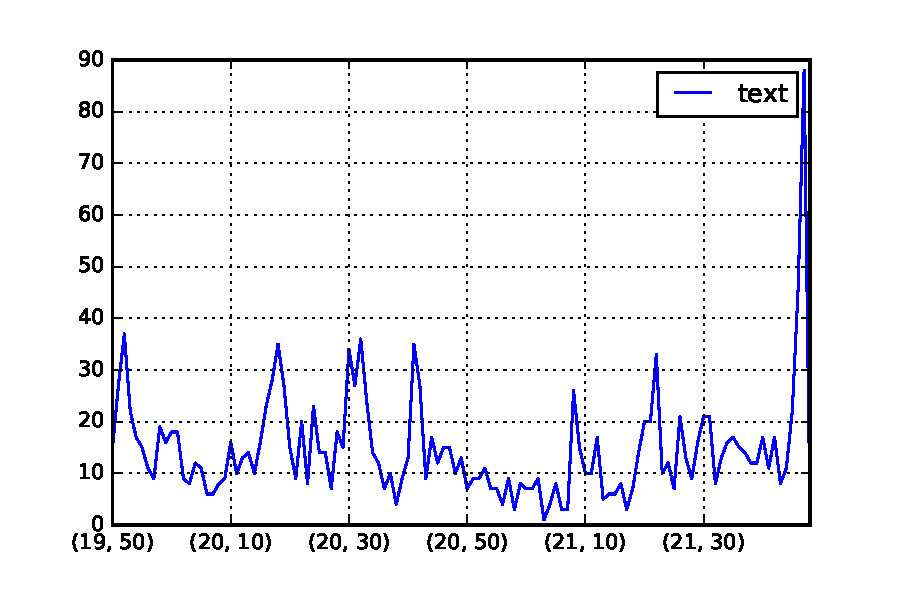
\includegraphics[width=0.12\linewidth]{OregonHC_clean_timeseries.pdf}
 }
 % Title
 {\sc\Huge Tweets and NCAA March Madness}
 % Authors
 {David Freed and Samuel Green\\[1em]
 {\texttt{davidfreed@college.harvard.edu, samuelgreen@college.harvard.edu}}}
 % University logo
 {
  \begin{tabular}{r}
    
\includegraphics[height=0.12\textheight]{logo}\\
  \end{tabular}
 }

%%%%%%%%%%%%%%%%%%%%%%%%%%%%%%%%%%%%%%%%%%%%%%%%%%%%%%%%%%%%%%%%%%%%%%%%%%%%%%
%%% Now define the boxes that make up the poster
%%%---------------------------------------------------------------------------
%%% Each box has a name and can be placed absolutely or relatively.
%%% The only inconvenience is that you can only specify a relative position 
%%% towards an already declared box. So if you have a box attached to the 
%%% bottom, one to the top and a third one which should be inbetween, you 
%%% have to specify the top and bottom boxes before you specify the middle 
%%% box.
%%%%%%%%%%%%%%%%%%%%%%%%%%%%%%%%%%%%%%%%%%%%%%%%%%%%%%%%%%%%%%%%%%%%%%%%%%%%%%

%%%%%%%%%%%%%%%%%%%%%%%%%%%%%%%%%%%%%%%%%%%%%%%%%%%%%%%%%%%%%%%%%%%%%%%%%%%%%%
  \headerbox{Real-Time Win Probability Modeling with Twitter}{name=abstract,column=0,row=0,span=2}{
%%%%%%%%%%%%%%%%%%%%%%%%%%%%%%%%%%%%%%%%%%%%%%%%%%%%%%%%%%%%%%%%%%%%%%%%%%%%%%
  This project investigates the predictive power of Twitter data in modeling the outcomes and events
  in NCAA March Madness basketball games. We extend previous work that used only pools of data
  collected in advance of games to make single-period predictions about outcomes, instead
  collecting live-action time series of tweets in-game. We find that the volumes of 
  relevant tweets far outpace the tweets collected in previous work and that tweet volumes
  appear to coincide with in-game events. {\bf Using basic models for online learning, we conclude
  that tweets can be used to improve over standard logistic regression models in making predictions
  about game events and outcomes. }
  }
%%%%%%%%%%%%%%%%%%%%%%%%%%%%%%%%%%%%%%%%%%%%%%%%%%%%%%%%%%%%%%%%%%%%%%%%%%%%%%
  \headerbox{Data Collection}{name=collection,column=0,below=abstract}{
%%%%%%%%%%%%%%%%%%%%%%%%%%%%%%%%%%%%%%%%%%%%%%%%%%%%%%%%%%%%%%%%%%%%%%%%%%%%%%
    Our dataset compiles approximately 1 million tweets from
    42 games during the NCAA March Madness. For each game, 
    we compiled hashtags relevant to the game, which we
    then used to collect tweets via the Streaming API. 
    An set of example hashtags is: 
    \begin{center}
    \#MarylandvsHawaii \#WeWill \#Maryland \#Terrapins \#RainbowWarriors \#Hawaii \#HawaiiMBB \#RoadWarriors \#GoBows
    \end{center}
    Summary statistics for the entire dataset are:
    \begin{center}
    \begin{tabular}{ccccc} 
    \\[-1.8ex]\hline 
    \hline \\[-1.8ex] 
     \multicolumn{1}{c}{N} & \multicolumn{1}{c}{Mean} & \multicolumn{1}{c}{St. Dev.} & \multicolumn{1}{c}{Min} & \multicolumn{1}{c}{Max} \\ 
    \hline \\[-1.8ex] 
    42 & 20,754.810 & 27,273.890 & 1,930 & 171,600 \\ 
    \hline \\[-1.8ex] 
    \end{tabular}
    \end{center}   
}



 %%%%%%%%%%%%%%%%%%%%%%%%%%%%%%%%%%%%%%%%%%%%%%%%%%%%%%%%%%%%%%%%%%%%%%%%%%%%%%
   \headerbox{Our methods are at the performance/speed sweet point}{name=speed,column=2,row=0,span=2}{
 %%%%%%%%%%%%%%%%%%%%%%%%%%%%%%%%%%%%%%%%%%%%%%%%%%%%%%%%%%%%%%%%%%%%%%%%%%%%%%
   \newlength{\MSZ}
   \setlength{\MSZ}{0.01\textwidth}
   \newcommand{\MarkerCircle}[1]{%
     \tikz{\draw[use as bounding box] (0,0); \draw[fill=#1]             circle(\MSZ);}}
   \newcommand{\MarkerRectangle}[1]{%
     \tikz{\draw[use as bounding box] (0,0); \draw[fill=#1]             (-\MSZ,-\MSZ) rectangle +(2\MSZ,2\MSZ);}}
   \newcommand{\MarkerDiamond}[1]{%
     \tikz{\draw[use as bounding box] (0,0); \draw[fill=#1,rotate=45]   rectangle +(2\MSZ,2\MSZ);}}
   \newcommand{\MarkerTriangle}[1]{%
     \tikz{\draw[use as bounding box] (0,0); \draw[fill=#1]             (-0.866\MSZ,-0.5\MSZ) -- (0\MSZ,1\MSZ) -- (0.866\MSZ,-0.5\MSZ) -- cycle ;}}
   \newcommand{\MarkerUDTriangle}[1]{%
     \tikz{\draw[use as bounding box] (0,0); \draw[fill=#1,rotate=180]  (-0.866\MSZ,-0.5\MSZ) -- (0\MSZ,1\MSZ) -- (0.866\MSZ,-0.5\MSZ) -- cycle ;}}
   \newcommand{\MarkerPlus}[1]{%
     \tikz{\draw[use as bounding box] (0,0); \draw[fill=#1]         (-\MSZ,-0.25\MSZ) rectangle +(2\MSZ,0.5\MSZ) (-0.25\MSZ,-\MSZ) rectangle +(0.5\MSZ,2\MSZ);}}
   \newcommand{\MarkerX}[1]{%
     \tikz{\draw[use as bounding box] (0,0); \draw[fill=#1,rotate=45]         (-\MSZ,-0.25\MSZ) rectangle +(2\MSZ,0.5\MSZ) (-0.25\MSZ,-\MSZ) rectangle +(0.5\MSZ,2\MSZ);}}
   \begin{tikzpicture}[x=0.00425\linewidth,y=13mm,font=\smaller]
     % Ticks
     \begin{scope}[color=black]
       \foreach \y in {-0.2218487496,-0.1549019600,-0.0969100130,-0.0457574906,0.0000000000,
                       0.0000000000,0.3010299957,0.4771212547,0.6020599913,0.6989700043,0.7781512504,0.8450980400,0.9030899870,0.9542425094,1.0000000000,
                       1.0000000000,1.3010299957,1.4771212547,1.6020599913,1.6989700043,1.7781512504,1.8450980400,1.9030899870,1.9542425094,2.0000000000,
                       2.0000000000,2.3010299957,2.4771212547,2.6020599913,2.6989700043,2.7781512504,2.8450980400,2.9030899870,2.9542425094,3.0000000000} {
         \draw[color=lightgray!20!white] (0,\y) -- +(100,0); 
       }
       \foreach \y/\lbl in {0/$10^0$,1/$10^1$,2/$10^2$,3/$10^3$} {
         \draw[color=black]     (0,\y) node[anchor=east,color=black] {\lbl} -- +(100,0); 
         \draw[color=lightgray] (0,\y) -- +(100,0); 
         \draw[color=black]     (0,\y) -- +(0.5\MSZ,0mm); 
       }
       \foreach \x in {0,20,40,60,80,100} {
         \draw (\x,-0.23) node[anchor=north,color=black] {\x};
         \draw[color=lightgray] (\x,-0.23) -- +(0,3.23);
         \draw[color=black] (\x,-0.23) -- +(0mm,0.5\MSZ);
       }
     \end{scope}
     % Border
     \draw[color=black] (0,3) -- (0,-0.23)  (100,-0.23) -- (100,3);
     % Axis labels
     \draw (50,-0.23)  node[below,yshift=-1em]{Success Rate (\%, Larger is better)};
     \draw (0,1.5) node[above,rotate=90,yshift=1.6em]{Runtime (smaller is better)};
     \draw (50,3)  node[above]{The main algorithms starting within $20\%$ \ied{}};
     % Data
     \foreach \anch/\rot/\xs/\ys/\x/\y/\ttl/\stl in {
     west/  0  / 1   / 0   /  5.2631578947   /     0.0000000000 /  Original \ICIA{}        / {\MarkerCircle{blue}},
   %  west/  0  / 1   / 0   / 14.2369727047   /     0.1128364125 /  \ICIA{} + V^{\text{norm}}/ {\MarkerCircle{blue!70!white}},
     east/  0  /-1   / 0   / 38.9423076923   /     0.8814699511 /  \CoLiNe{}                / {\MarkerRectangle{green}},
     west/  0  / 1   / 0   / 39.4696029777   /     0.2610806897 /  \LinCoDe{}               / {\MarkerTriangle{red}},
     west/  0  / 1   / 0   / 56.8548387097   /     0.9091243545 /  \CoDe{}                  / {\MarkerUDTriangle{yellow}},
     west/  0  / 1   / 0   / 36.4299007444   /     1.3563671940 /  \CoNe{}                  / {\MarkerX{black!50!white}},
     west/  0  / 1   / 0   / 41.6918429003   /     2.6132022326 /  L-BFGS (with reg)     / {\MarkerPlus{red!50!blue!50!black}}
     }{
       \draw (\x,\y) 
         node[fill=none,anchor=\anch,xshift=\xs\MSZ,yshift=\ys\MSZ,rotate=\rot] {\ttl} 
         node{\stl};
       \draw[fill=black] (\x,\y) circle(0.3\MSZ);
     }
   \end{tikzpicture}
   \begin{tikzpicture}[x=0.00425\linewidth,y=13mm,font=\smaller]
     % Ticks
     \begin{scope}[color=black]
       \foreach \y in {-0.2218487496,-0.1549019600,-0.0969100130,-0.0457574906,0.0000000000,
                       0.0000000000,0.3010299957,0.4771212547,0.6020599913,0.6989700043,0.7781512504,0.8450980400,0.9030899870,0.9542425094,1.0000000000,
                       1.0000000000,1.3010299957,1.4771212547,1.6020599913,1.6989700043,1.7781512504,1.8450980400,1.9030899870,1.9542425094,2.0000000000,
                       2.0000000000,2.3010299957,2.4771212547,2.6020599913,2.6989700043,2.7781512504,2.8450980400,2.9030899870,2.9542425094,3.0000000000} {
         \draw[color=lightgray!20!white] (0,\y) -- +(100,0); 
       }
       \foreach \y/\lbl in {0/$10^0$,1/$10^1$,2/$10^2$,3/$10^3$} {
         \draw[color=black]     (0,\y) node[anchor=east,color=black] {\lbl} -- +(100,0); 
         \draw[color=lightgray] (0,\y) -- +(100,0); 
         \draw[color=black]     (0,\y) -- +(0.5\MSZ,0mm); 
       }
       \foreach \x in {0,20,40,60,80,100} {
         \draw (\x,-0.23) node[anchor=north,color=black] {\x};
         \draw[color=lightgray] (\x,-0.23) -- +(0,3.23);
         \draw[color=black] (\x,-0.23) -- +(0mm,0.5\MSZ);
       }
     \end{scope}
     % Border
     \draw[color=black] (0,3) -- (0,-0.23)  (100,-0.23) -- (100,3);
     % Axis labels
     \draw (50,-0.23)  node[below,yshift=-1em]{Success Rate (\%, Larger is better)};
     \draw (0,1.5) node[above,rotate=90,yshift=1.6em]{Runtime (smaller is better)};
     \draw (50,3)  node[above,text width=0.5\linewidth,text centered]{All algorithms with $V^{\text{norm}}$ and regularisation};

     \foreach \anch/\rot/\xs/\ys/\x/\y/\ttl/\stl in {
       south/0 / 0   /  1.0/       26.4701318852 /         0.6174735535 / \ICIA{} + $V^{\text{norm}}$ / {\MarkerCircle{    blue!50!black}},
       south/0 / 0   /  1.0/       52.1334367727 /         1.0781366795 / \CoLiNe{}   / {\MarkerRectangle{ green!50!black}},
       west/ 0 / 1   /  0  /       55.9348332040 /         0.5514820720 / \LinCoDe{}  / {\MarkerTriangle{  red!50!black}},
       west/ 0 / 1   /  0  /       66.0356865787 /         1.1158139989 / \CoDe{}     / {\MarkerUDTriangle{yellow!50!black}},
       west/ 0 / 1   /  0  /       66.9511249030 /         1.8260835334 / \CoNe{}     / {\MarkerX{         black!50!white!50!black}},
       west/ 0 / 1   /  0  /       41.6918429003 /         2.6132022326 / L-BFGS   / {\MarkerPlus{      red!50!blue!50!black}}
     }{
       \draw (\x,\y) 
         node[fill=none,anchor=\anch,xshift=\xs\MSZ,yshift=\ys\MSZ,rotate=\rot] {\ttl} 
         node{\stl};
       \draw[fill=black] (\x,\y) circle(0.3\MSZ);
     }
   \end{tikzpicture}
   \begin{multicols}{2}
   \textbf{Fitting a multiperson AAM. }
   The best speed--performance tradeoffs come from the two new algorithms
   \CoDe{} and \LinCoDe{}. Note that \ICIA{} is practically useless on
   this difficult multi-person dataset with a success rate near zero (left). It
   can be improved (right) by using the orthonormal incremental warp and
   regularisation. The \CoDe{} algorithm with regularisation (right) is as
   accurate as the slow, approximation-free, compositional Gauss-Newton \CoNe{}
   method but is seven times more efficient.

   The experiments were performed with leave one identity out on a mixture of two databases (XM2VTS and IMM).
   \end{multicols}
   }

%%%%%%%%%%%%%%%%%%%%%%%%%%%%%%%%%%%%%%%%%%%%%%%%%%%%%%%%%%%%%%%%%%%%%%%%%%%%%%
%   \headerbox{Methods Compared}{name=methods,column=0}{
% %%%%%%%%%%%%%%%%%%%%%%%%%%%%%%%%%%%%%%%%%%%%%%%%%%%%%%%%%%%%%%%%%%%%%%%%%%%%%%
%   \begin{tabular}{rllllll}
%     Method                              & Hessian               &                                        & Gradient        &                                  & Speed      & Capture Range\\
%     \midrule
% \CoDe{} (this paper)                & Not used              &                                        & True:           & $\tilde{J}_{\qq_0}^T\e{\qq_0}$   & Fast       & Large  \\[0.1em]
% \LinCoDe{} (this paper)             & Not used              &                                        & Linear Approx:  & $\bar{J}^T\e{\qq_0}$             & Very Fast  & Medium \\[0.1em]
% \CoLiNe{}~\cite{burkhardt86:motion} & Constant Approx.:     & $\bar{J}^T\bar{J}$                     & True:           & $\tilde{J}_{\qq_0}^T\e{\qq_0}$   & Fast       & Medium \\[0.1em]
% \ICIA{}~\cite{matthews:aamr}        & Constant Approx.:     & $\bar{J}^T\bar{J}$                     & Linear Approx:  & $\bar{J}^T\e{\qq_0}$             & Very Fast  & Small  \\[0.1em]
% \CoNe{}~\cite{matthews:kanade20}    & Gauss-Newton Approx.: & $\tilde{J}_{\qq_0}^T\tilde{J}_{\qq_0}$ & True:           & $\tilde{J}_{\qq_0}^T\e{\qq_0}$   & Slow       & Large  
%   \end{tabular}
%   The methods introduced in this paper are Hessian-free gradient descent methods.
%  }
%
 %%%%%%%%%%%%%%%%%%%%%%%%%%%%%%%%%%%%%%%%%%%%%%%%%%%%%%%%%%%%%%%%%%%%%%%%%%%%%%
   \headerbox{References}{name=references,column=0,above=bottom}{
 %%%%%%%%%%%%%%%%%%%%%%%%%%%%%%%%%%%%%%%%%%%%%%%%%%%%%%%%%%%%%%%%%%%%%%%%%%%%%%
     \smaller
     
     \bibliographystyle{ieee}
     \renewcommand{\section}[2]{\vskip 0.05em}
       \begin{thebibliography}{1}\itemsep=-0.01em
       \setlength{\baselineskip}{0.4em}

       \bibitem{amberg07:nicp}
       B.~Amberg, A.~Blake, T.~Vetter
       \newblock On Compositional Image Alignment with an Application to Activce Appearance Models
       \newblock In {\em CVPR'09}, 2009.

       \end{thebibliography}
   }

 %%%%%%%%%%%%%%%%%%%%%%%%%%%%%%%%%%%%%%%%%%%%%%%%%%%%%%%%%%%%%%%%%%%%%%%%%%%%%%
   \headerbox{Training + Testing Data}{name=data,column=0,above=references,below=collection}{
 %%%%%%%%%%%%%%%%%%%%%%%%%%%%%%%%%%%%%%%%%%%%%%%%%%%%%%%%%%%%%%%%%%%%%%%%%%%%%%
   % 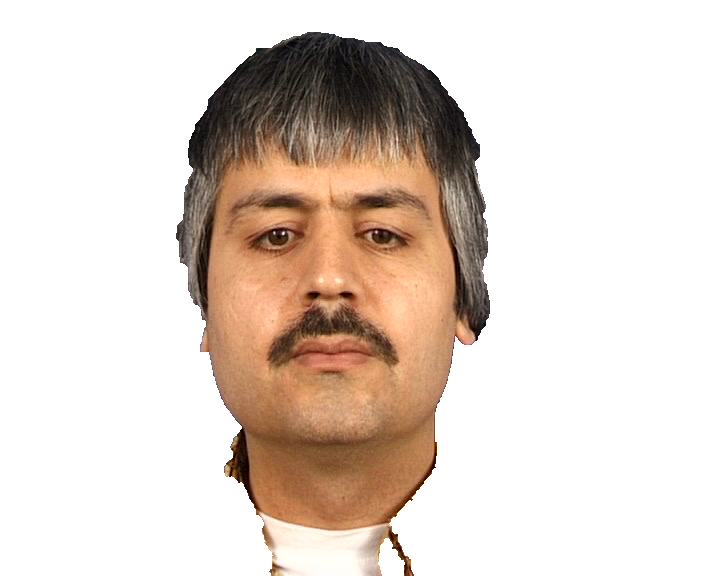
\includegraphics[width=0.2\linewidth]{018_4_2_masked}%
   % 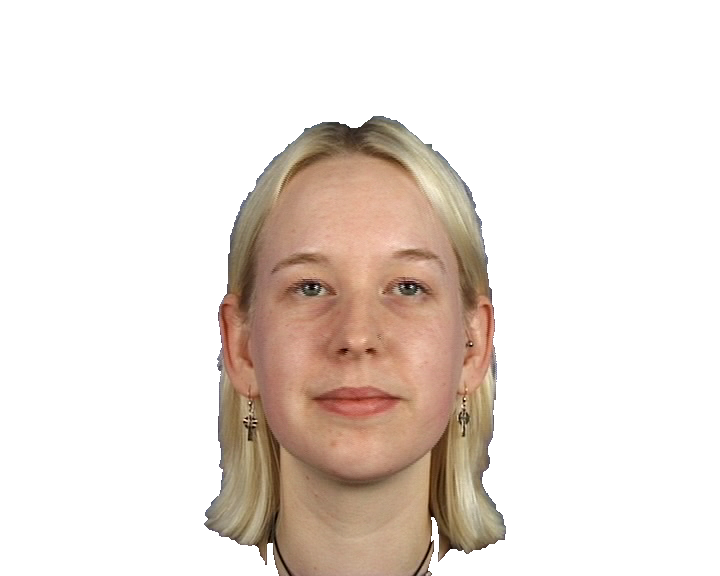
\includegraphics[width=0.2\linewidth]{328_2_1_masked}%
   % 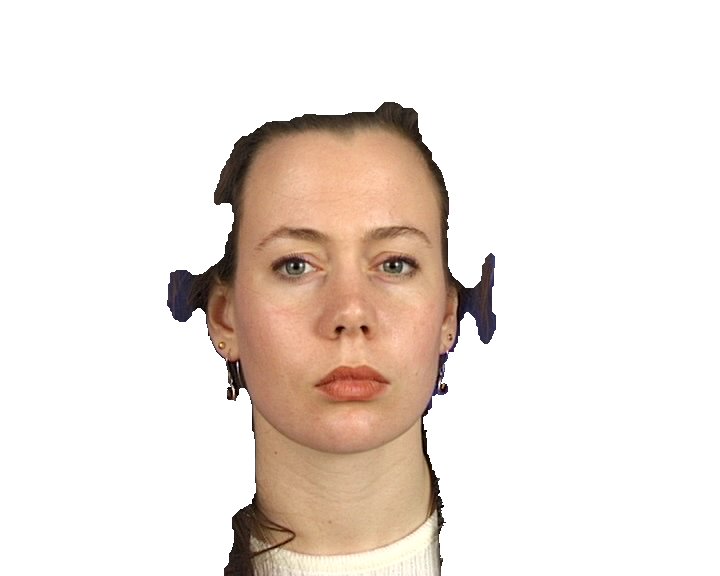
\includegraphics[width=0.2\linewidth]{319_2_1_masked}%
   % 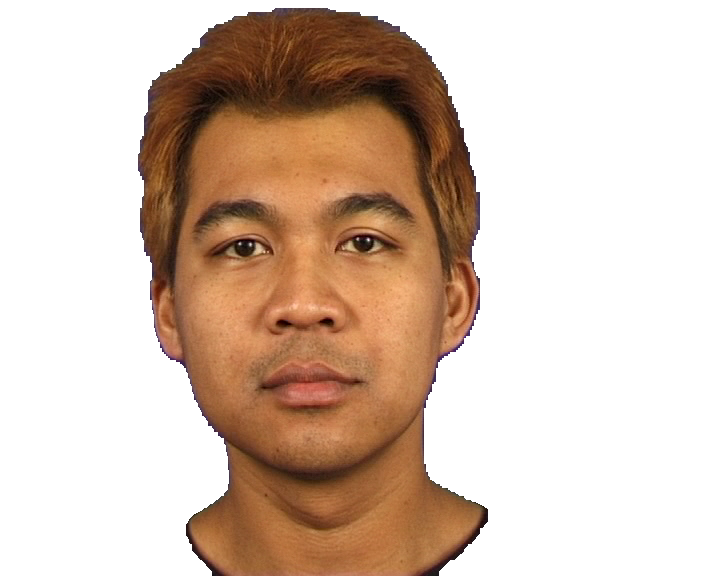
\includegraphics[width=0.2\linewidth]{027_4_2_masked}%
   % 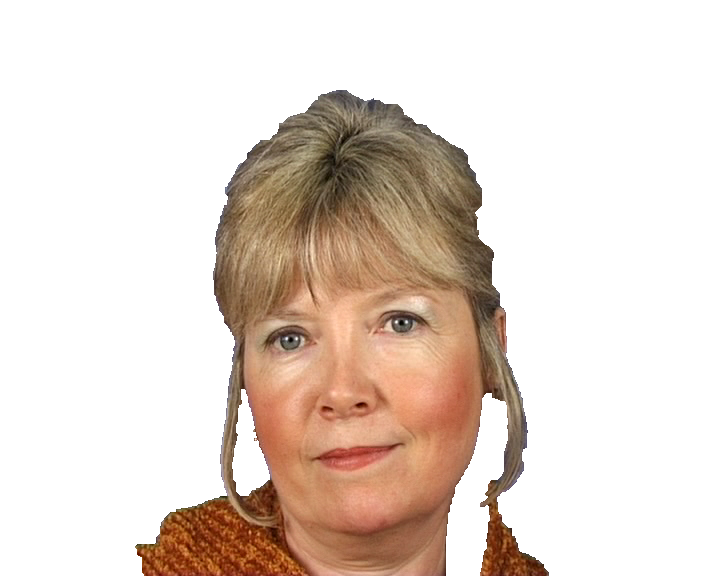
\includegraphics[width=0.2\linewidth]{020_1_1_masked}
   % 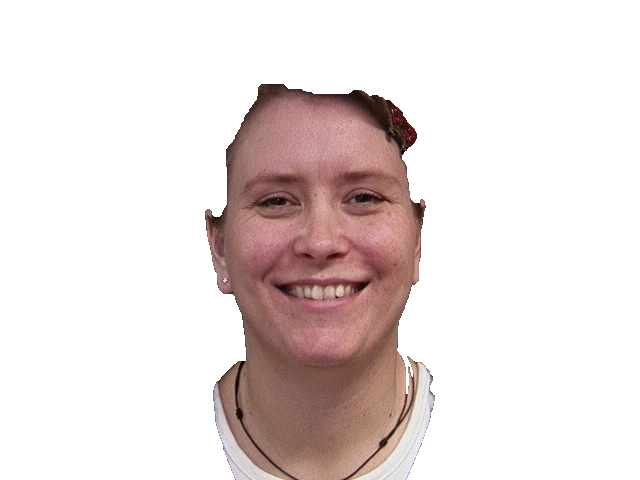
\includegraphics[width=0.2\linewidth]{12_2f_masked}%
   % 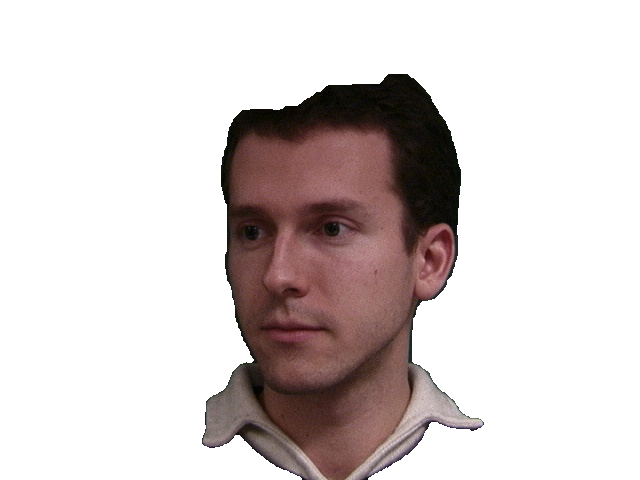
\includegraphics[width=0.2\linewidth]{21_3m_masked}%
   % 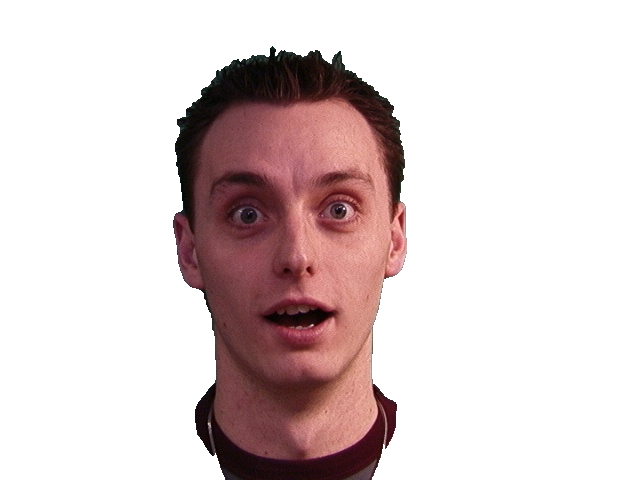
\includegraphics[width=0.2\linewidth]{09_6m_masked}%
   % 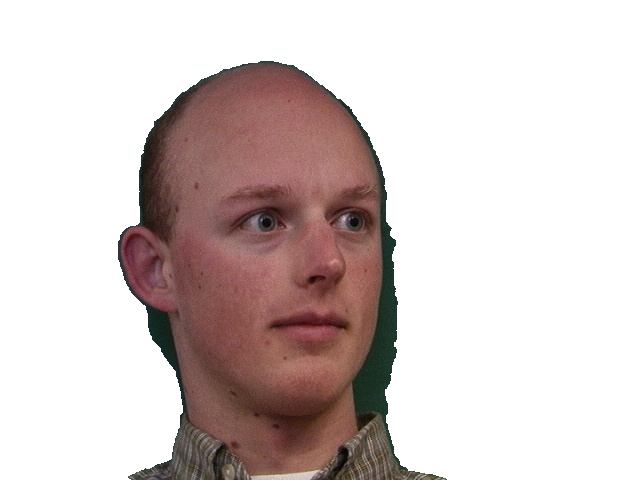
\includegraphics[width=0.2\linewidth]{33_4m_masked}%
   %\includegraphics[width=0.2\linewidth]{22_3f_masked}
   $\dots$\\
   The model was trained from 456 images from the IMM and XM2VTS datasets using
   120 landmarks. Get the landmarks, model, and source code at:\\
   \mbox{\url{www.cs.unibas.ch/personen/amberg_brian/aam/}}
   }

 %%%%%%%%%%%%%%%%%%%%%%%%%%%%%%%%%%%%%%%%%%%%%%%%%%%%%%%%%%%%%%%%%%%%%%%%%%%%%%

   \headerbox{Tracking 5000 frames with a general model}{name=tracking,column=2,span=2,below=speed,above=bottom}{
 %%%%%%%%%%%%%%%%%%%%%%%%%%%%%%%%%%%%%%%%%%%%%%%%%%%%%%%%%%%%%%%%%%%%%%%%%%%%%%
 {
 \begin{tabular}{c@{\hspace{0.05em}}c@{\hspace{0.1em}}c@{\hspace{0.1em}}c@{\hspace{0.1em}}c@{\hspace{1em}}c@{\hspace{0.1em}}c@{\hspace{0.1em}}c@{\hspace{0.1em}}c@{\hspace{0.1em}}c}
   \multicolumn{5}{c}{\smaller \ICIA{} with $\VLins$} &
   \multicolumn{5}{c}{\smaller \ICIA{} with $\VLins$ + Regularisation}\\[-0.2em]
   % 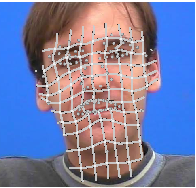
\includegraphics[width=0.095\linewidth]{track_frame_00010_01}&
   % 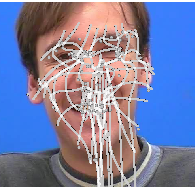
\includegraphics[width=0.095\linewidth]{track_frame_00050_01}&
   % 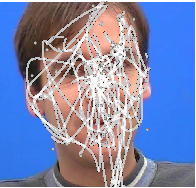
\includegraphics[width=0.095\linewidth]{track_frame_00450_01}&
   % 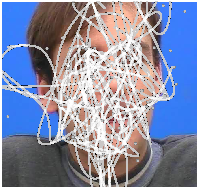
\includegraphics[width=0.095\linewidth]{track_frame_02000_01}&
   % 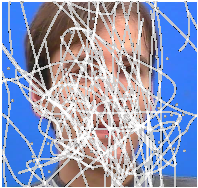
\includegraphics[width=0.095\linewidth]{track_frame_04999_01}&
   % %
   % 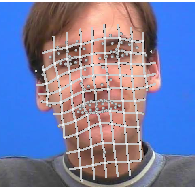
\includegraphics[width=0.095\linewidth]{track_frame_00010_02}&
   % 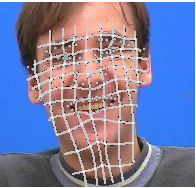
\includegraphics[width=0.095\linewidth]{track_frame_00050_02}&
   % 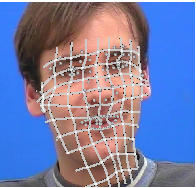
\includegraphics[width=0.095\linewidth]{track_frame_00450_02}&
   % 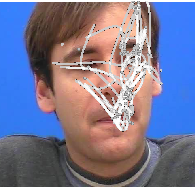
\includegraphics[width=0.095\linewidth]{track_frame_02000_02}&
   % 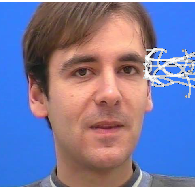
\includegraphics[width=0.095\linewidth]{track_frame_04999_02}\\[-0.1em]
   % %
   % \multicolumn{5}{c}{\smaller \LinCoDe{}} &
   % \multicolumn{5}{c}{\smaller \LinCoDe{} + Regularisation}\\[-0.2em]
   % 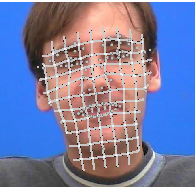
\includegraphics[width=0.095\linewidth]{track_frame_00010_03}&
   % 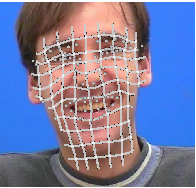
\includegraphics[width=0.095\linewidth]{track_frame_00050_03}&
   % 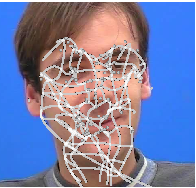
\includegraphics[width=0.095\linewidth]{track_frame_00450_03}&
   % 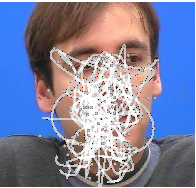
\includegraphics[width=0.095\linewidth]{track_frame_02000_03}&
   % 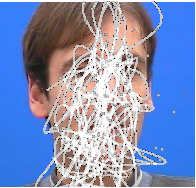
\includegraphics[width=0.095\linewidth]{track_frame_04999_03}&
   % %
   % 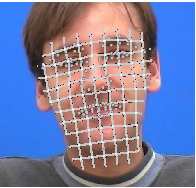
\includegraphics[width=0.095\linewidth]{track_frame_00010_04}&
   % 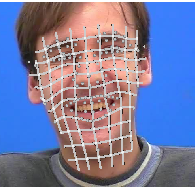
\includegraphics[width=0.095\linewidth]{track_frame_00050_04}&
   % 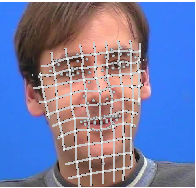
\includegraphics[width=0.095\linewidth]{track_frame_00450_04}&
   % 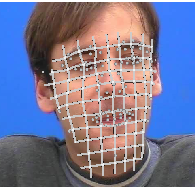
\includegraphics[width=0.095\linewidth]{track_frame_02000_04}&
   % 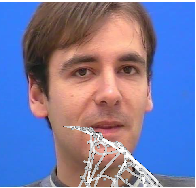
\includegraphics[width=0.095\linewidth]{track_frame_04999_04}\\[-0.1em]
   % %
   % \multicolumn{5}{c}{\smaller \CoDe{}} &
   % \multicolumn{5}{c}{\smaller \CoDe{} + Regularisation}\\[-0.2em]
   % 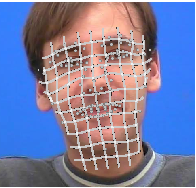
\includegraphics[width=0.095\linewidth]{track_frame_00010_05}&
   % 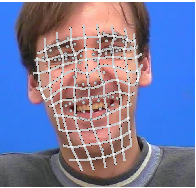
\includegraphics[width=0.095\linewidth]{track_frame_00050_05}&
   % 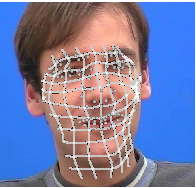
\includegraphics[width=0.095\linewidth]{track_frame_00450_05}&
   % 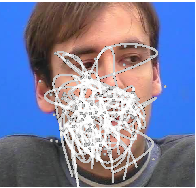
\includegraphics[width=0.095\linewidth]{track_frame_02000_05}&
   % 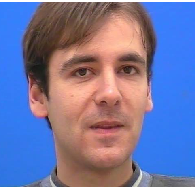
\includegraphics[width=0.095\linewidth]{track_frame_04999_05}&
   % %
   % 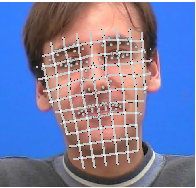
\includegraphics[width=0.095\linewidth]{track_frame_00010_06}&
   % 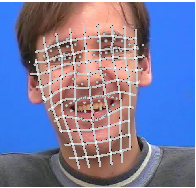
\includegraphics[width=0.095\linewidth]{track_frame_00050_06}&
   % 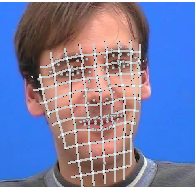
\includegraphics[width=0.095\linewidth]{track_frame_00450_06}&
   % 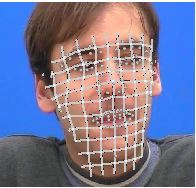
\includegraphics[width=0.095\linewidth]{track_frame_02000_06}&
   % 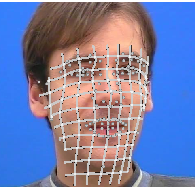
\includegraphics[width=0.095\linewidth]{track_frame_04999_06}\\[-0.5em]
   \smaller Frame 10 & \smaller Frame 50 & \smaller Frame 450 & \smaller Frame 2000 & \smaller Frame 5000 &
   \smaller Frame 10 & \smaller Frame 50 & \smaller Frame 450 & \smaller Frame 2000 & \smaller Frame 5000
   \end{tabular}
 }
   \vspace{-1.2em}
   \begin{multicols}{2}
   {\textbf{Our algorithm makes fast and robust tracking possible.}
     We compare face tracking under natural motion, using \ICIA{},
     \LinCoDe{} and \CoDe{}. The original \ICIA{} fails
     immediately with this large model and new face data. Substituting the orthonormal
     incremental warp for the original \ICIA{} warp, the algorithm still loses track
     very early, whereas \LinCoDe{} and \CoDe{} can track much
     further. Finally, adding regularisation to all algorithms, \ICIA{} still
     loses track completely after approximately 500 frames and does not recover
     the local deformations accurately. In contrast \CoDe{} now tracks the full
     5000 frame sequence without reinitialization, and \LinCoDe{} tracks for 2500 frames.}
   
   The same training dataset was used for both tracking experiments. The
   training data was aquired with different camera and light settings from
   different subjects.
   \end{multicols}
   }
%  %%%%%%%%%%%%%%%%%%%%%%%%%%%%%%%%%%%%%%%%%%%%%%%%%%%%%%%%%%%%%%%%%%%%%%%%%%%%%%
   \headerbox{Low Res Tracking}{name=lowrestracking,column=1,span=1,above=bottom}{
%  %%%%%%%%%%%%%%%%%%%%%%%%%%%%%%%%%%%%%%%%%%%%%%%%%%%%%%%%%%%%%%%%%%%%%%%%%%%%%%
% \begin{tabular}{@{}c@{}c@{}c@{}c@{}c@{}}
%   \multicolumn{5}{c}{\smaller \ICIA{} with $\VLins$}\\[-0.2em]
%   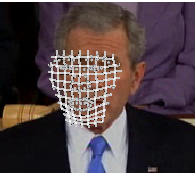
\includegraphics[width=0.2\linewidth]{bush_00010_02}&
%   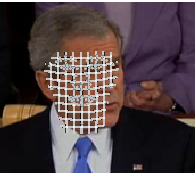
\includegraphics[width=0.2\linewidth]{bush_00100_02}&
%   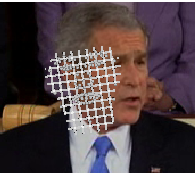
\includegraphics[width=0.2\linewidth]{bush_00200_02}&
%   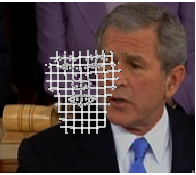
\includegraphics[width=0.2\linewidth]{bush_00300_02}&
%   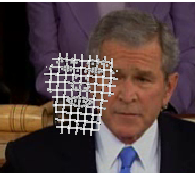
\includegraphics[width=0.2\linewidth]{bush_00400_02}\\[-0.1em]
%   \multicolumn{5}{c}{\smaller \LinCoDe{}}\\[-0.2em]
%   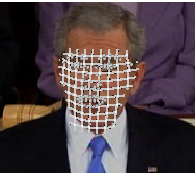
\includegraphics[width=0.2\linewidth]{bush_00010_05}&
%   \includegraphics[width=0.2\linewidth]{bush_00100_05}&
%   \includegraphics[width=0.2\linewidth]{bush_00200_05}&
%   \includegraphics[width=0.2\linewidth]{bush_00300_05}&
%   \includegraphics[width=0.2\linewidth]{bush_00400_05}\\[-0.1em]
%   \multicolumn{5}{c}{\smaller \CoDe{}}\\[-0.2em]
%   \includegraphics[width=0.2\linewidth]{bush_00010_08}&
%   \includegraphics[width=0.2\linewidth]{bush_00100_08}&
%   \includegraphics[width=0.2\linewidth]{bush_00200_08}&
%   \includegraphics[width=0.2\linewidth]{bush_00300_08}&
%   \includegraphics[width=0.2\linewidth]{bush_00400_08}\\[-0.5em]
%   \smaller Frame 10 & \smaller Frame 100 & \smaller Frame 200 & \smaller Frame 300 & \smaller Frame 400 
%   \end{tabular}

  \vspace{1.25em}
  \textbf{Tracking a low resolution video with large head motions
  succeeds with \CoDe{}, where \ICIA{} fails.}\\ All methods used the orthonormal
  incremental warp, and relatively strong regularisation.  \ICIA{} starts to
  drift in the early frames, while~\CoDe{} tracks the full sequence. The
  approximate gradient method \LinCoDe{} also suceeds, but looses
  track of the details for about 100 frames.
   }

 %%%%%%%%%%%%%%%%%%%%%%%%%%%%%%%%%%%%%%%%%%%%%%%%%%%%%%%%%%%%%%%%%%%%%%%%%%%%%%%
  \headerbox{Sentiment Analysis}{name=algorithm,column=1,below=abstract}{
 %%%%%%%%%%%%%%%%%%%%%%%%%%%%%%%%%%%%%%%%%%%%%%%%%%%%%%%%%%%%%%%%%%%%%%%%%%%%%%%
    As input to the model, we built a bag-of-words sentiment classifier using
    a labeled corpus of 4000 tweets. The classifer then uses a Naive-Bayes
    model to perform classfication after it has been trained using the labeled
    corpus. This training presents a problem to the analysis, since the classifier
    is trained on a set of tweets related to a different topic. 

    In order to use productively used the data to update the win probability
    model, we also had to associate the sentiment of the tweet with
    one or both teams. 
   }
   %%%%%%%%%%%%%%%%%%%%%%%%%%%%%%%%%%%%%%%%%%%%%%%%%%%%%%%%%%%%%%%%%%%%%%%%%%%%%%%
  \headerbox{Relevance Analysis}{name=relevance,column=1,above=lowrestracking,below=algorithm}{
 %%%%%%%%%%%%%%%%%%%%%%%%%%%%%%%%%%%%%%%%%%%%%%%%%%%%%%%%%%%%%%%%%%%%%%%%%%%%%%%
    As input to the model, we built a bag-of-words sentiment classifier using
    a labeled corpus of 4000 tweets. The classifer then use a Naive Bayes
    model to perform classfication after training. 

    In order to use productively used the data to update the win probability
    model, we also had to associate the sentiment of the tweet with
    one or both teams. 
   }

\end{poster}%
%
\end{document}
